% !TeX spellcheck = en_GB

\section{Architecture}\label{sec:architecture}

\subsection{Scenarios}
\label{sec:scenarios}
This document describes various scenarios of system usage and possible failures.

\subsubsection{Create Backup}\label{sec:scenario-create-backup}
The client wants to create a backup.

\begin{figure}[h]
    \centering
    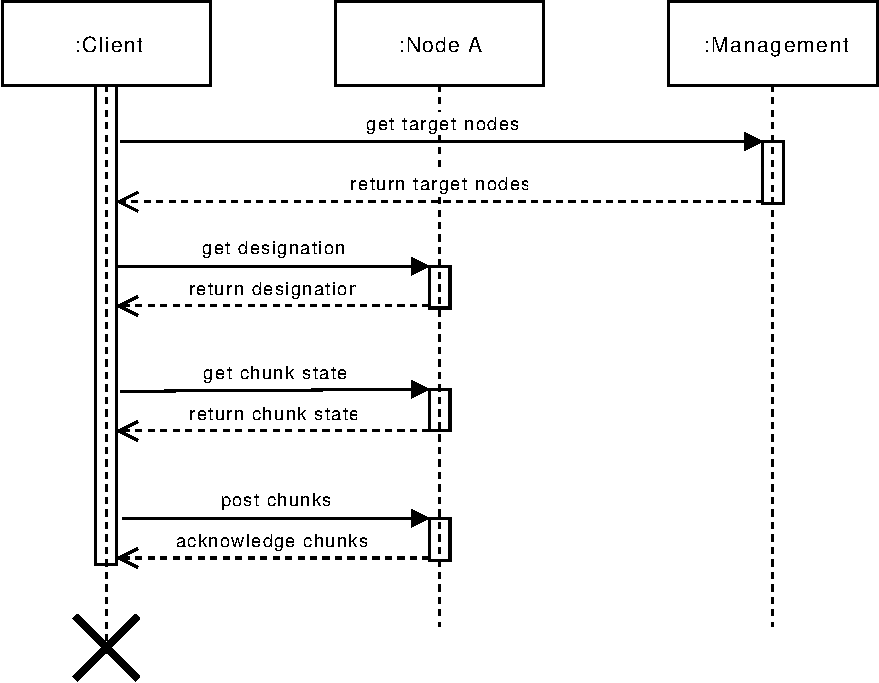
\includegraphics[width=\linewidth]{resources/create_backup}
    \caption{Create Backup Sequence Diagram}
    \label{fig:create-backup}
\end{figure}

\begin{enumerate}
    \item Client asks the management for a list of \emph{node}s. The \emph{management} returns a sorted list of all nodes (message: \emph{client fetch target nodes}) (sorting might be based on specific configuration).
        \begin{itemize}
            \item If the management is down and this is a first time backup, client records message and aborts.
            \item If the management is down, client tries the same host configuration as last time.
        \end{itemize}
    \item Client tries to contact nodes in the presorted order.
        \begin{enumerate}
            \item The client sends a \emph{client backup request}. %TODO: Define backup request with estimate, identification, how long the data should be stored
            \item The node acknowledges or denies the backup request.
            \item If the node acknowledges, it is declared as \emph{designated node}
            \item If the node denies the backup request, try next node.
            \item If no node answers the request, client records an error message and aborts.
       \end{enumerate}
   \item If the contact was established, the client starts creating a backup.
        \begin{enumerate}
            \item Split all files that changed since the last backup into \emph{chunk}s\footnote{using a rolling hash, see \url{https://borgbackup.readthedocs.io/en/stable/internals/data-structures.html\#chunks}} and calculate a corresponding hash, the \emph{chunk identifier} and add it to the local \emph{chunk index}.
            \item Files that have not changed since the last backup, must already be present in the chunk index.
            \item Send all chunk identifiers present in the chunk index combined with an \emph{expiration date} to the designated node. (message: \emph{client sends chunk list})
            \item The designated node checks, if all chunks received from the client chunk list are present on the node.
                \begin{itemize}
                    \item If a chunk is already present, update its expiration date if it is further in the future.
                    \item If a chunk is not present, request it from the client (see message response \emph{client sends chunk list} for further details)
                \end{itemize}
            \item The client sends the requested chunks to the designated node with a \emph{client sends chunks} message. %TODO: Abschluss client transaktion (root handle)
                \begin{enumerate}
                    \item The designated node verifies and persists the chunk into its \emph{storage}. Afterwards, it acknowledges receipt to the client (see \emph{client sends chunks} response message).
                                   %TODO: Client must remember, which chunks have been acknowledged. This could be done with a sliding window for QoS/memory usage?
                    \item The designated node replicates chunks in a continuous replication process. (See scenario~\ref{sec:scenario-data-replication})
                \end{enumerate}
            \item The client creates a \emph{serialised metadata chunks}. %TODO: Serialised Metadata is the chunk index plus backup metadata as linked list
            \item The client sends the additional chunks (as \emph{client sends chunk list} messages) to the designated node, in which the \emph{root handle} is highlighted. %TODO: The root handle holds a reference to the first list chunk as well as owner etc. information.
        \end{enumerate}
\end{enumerate}

\paragraph{Special cases}
\begin{itemize}
    \item If a client is suspended while running, it continuous with the backup process on resume. %TODO: If the expiration date is in the past, the node should refuse the chunk.
    \item If a file is changed while the backup is running, and the chunk cannot be created, the backup must be restarted. %TODO: This may lead to starvation.
    \item If client crashes, the backup is aborted and won't be continued if the client is restarted.
    \item If the node goes away (disconnects/crashes/shuts down) during the backup, the client tries to resume the process. After a certain time (e.g. 15m), the client gives up and restarts the backup process from the beginning.
    \item The node must reject (i.e.\ not acknowledge) a chunk, if the creation date is more than e.g.\ an hour in the future or past to prevent data loss on bad synchronized clocks.
    \item If the node runs out of storage capacity, it does reject further data chunks. After a timeout, the client restarts the backup process (with another designated node).
\end{itemize}

\paragraph{Possible simplifications in this study project}
\begin{description}
    \item[3a)] Don't split files into chunks, send them as is.
\end{description}

\subsubsection{Backup Restore}\label{sec:scenario-backup-restore}
The client wants to restore specific data.

\begin{figure}[h]
    \centering
    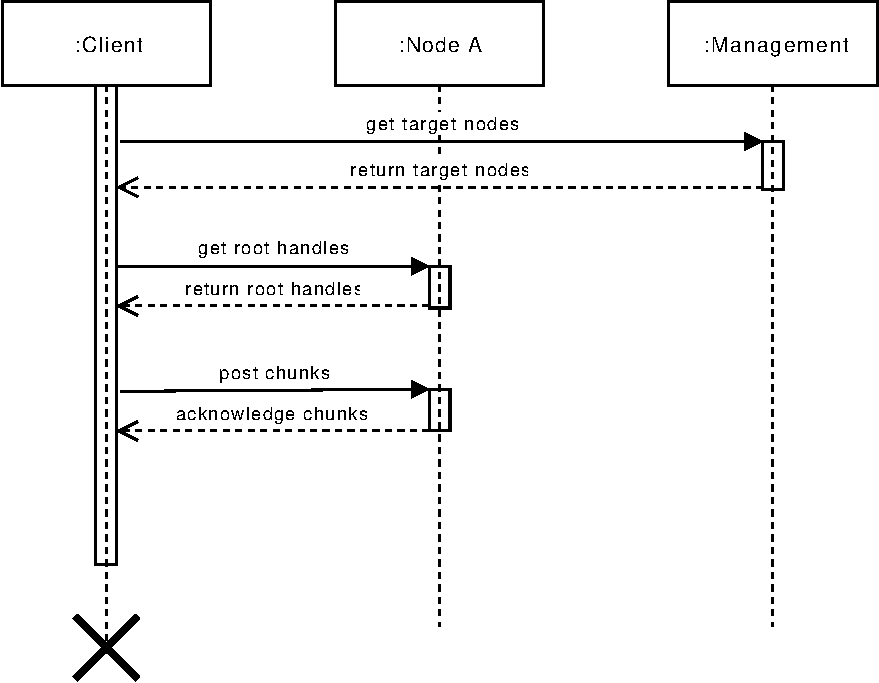
\includegraphics[width=\linewidth]{resources/backup_restore.pdf}
    \caption{Backup Restore Sequence Diagram}
    \label{fig:backup-restore}
\end{figure}

\begin{enumerate}
    \item See scenario~\ref{sec:scenario-create-backup} step 1.
    \item The client contacts nodes in the presorted order
        \begin{enumerate}
            \item The client sends a \emph{client list root handles} requests to a node.
            \item The node returns all root handles present in the system (see \emph{client list root handles} response message)
            \item If no node answers the request, client records an error message and aborts.
        \end{enumerate}
    \item The client fetches all \emph{serialised metadata chunks} from the chosen node (message: \emph{client fetch chunks}) and reassembles \emph{chunk index} and backup metadata.
    \item The user specifies which files in which backup version shall be restored. %TODO: Use snapshot as single backup name?
    \item Based on the specified files, the client looks up the \emph{chunk identifiers} in the corresponding \emph{chunk index}.
    \item The client requests the \emph{chunks} from the selected node. (message: \emph{client fetch chunks})
    \item The client reassembles the chunks into files.
\end{enumerate}

\paragraph{Special cases}
\begin{itemize}
    \item If the selected node does not hold the requested chunk, it requests it recursively.
    \item If the client crashes, the whole restore process must be repeated
    \item If the selected node is unavailable, the client selects a new node after a certain timeout (e.g.\ 5m)
\end{itemize}

\paragraph{Possible simplifications in this study project}
\begin{description}
    \item[-] The client must request a node that has the data already available (possibly the node where the backup was created).
\end{description}


\subsubsection{Node Joining}\label{sec:scenario-node-join}
A new node joins the system.

\begin{figure}[h]
    \centering
    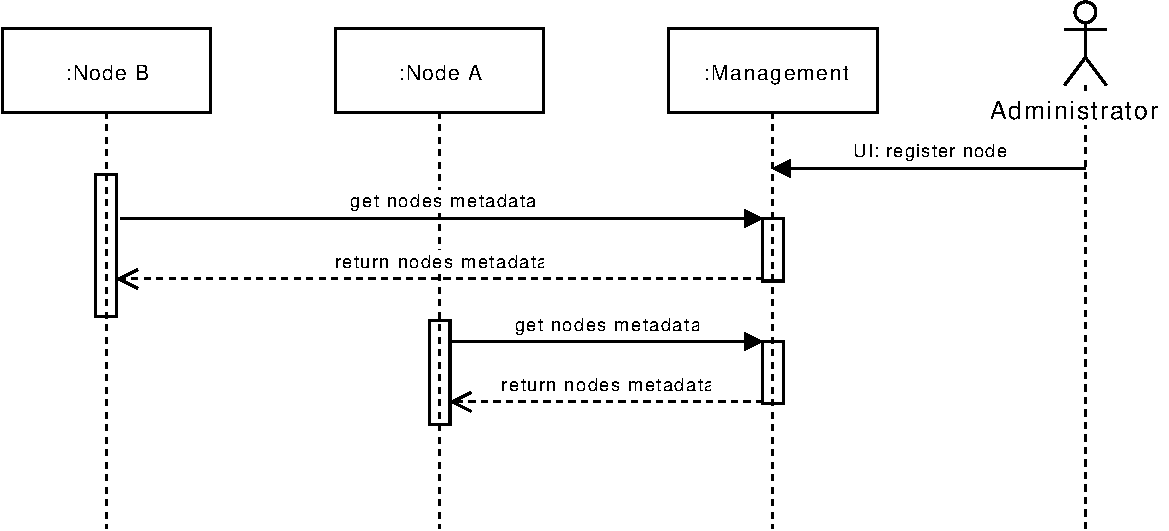
\includegraphics[width=\linewidth]{resources/node_joining.pdf}
    \caption{Node Joining Sequence Diagram}
    \label{fig:node-joining}
\end{figure}

This scenario is described as it is implemented in the study project. It might be subject to further evaluation in the future.

\begin{enumerate}
    \item The node is registered by an administrator in the \emph{managment} using its \emph{node identifier}. A \emph{location} must also be assigned to the node. %TODO: Data
    \item The new node queries information of all nodes from the management (message: \emph{node fetch all nodes metadata}) on startup. 
    \item The new node configures itself based on its \emph{node identifier} and the response from the management.
        \begin{itemize}
            \item If the management has no information available (yet) or is unavailable, the node retries after a certain timeout (e.g.\ 5min).
        \end{itemize}
    \item Other nodes learn about the new node through periodical metadata queries (message: \emph{node fetch all nodes metadata}) %TODO: Component description: regular queries
        \begin{enumerate}
            \item If the new host contacts an existing node, before the existing node updates its metadata, the existing node should query the management (message: \emph{node fetch all nodes metadata})
            \item If the management is unavailable, the node ignores all communication attempts.
        \end{enumerate}
\end{enumerate}

\subsubsection{Node Leaving Planned}\label{sec:scenario-node-leave-planned}
A node leaves the system planned

\begin{figure}[h]
    \centering
    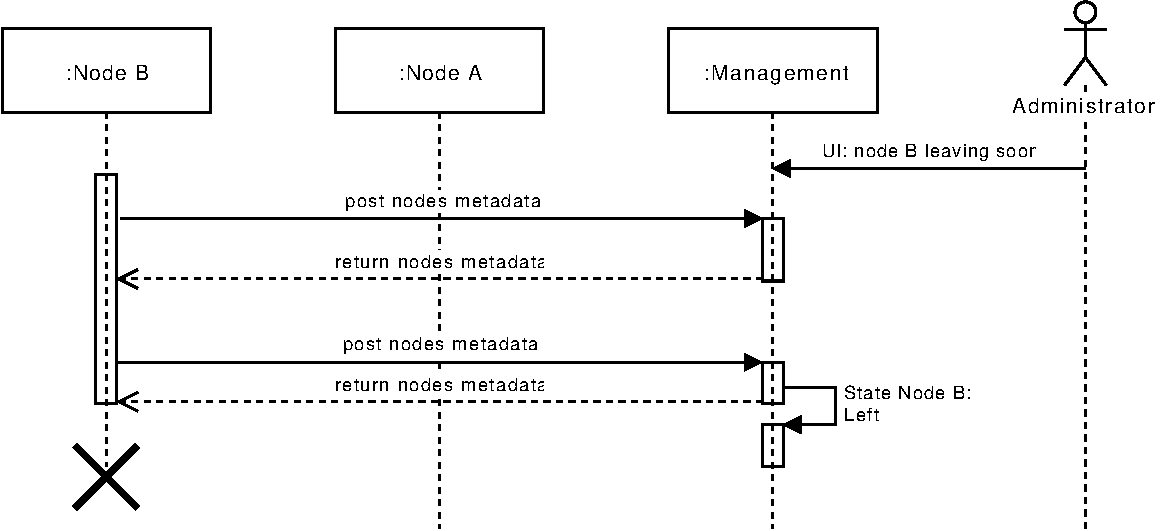
\includegraphics[width=\linewidth]{resources/node_leaving_planned.pdf}
    \caption{Node Leaving Planned Sequence Diagram}
    \label{fig:node-leave-planned}
\end{figure}

This scenario is described as it is implemented in the study project. It might be subject to further evaluation in the future.

\begin{enumerate}
    \item The node is marked as \emph{leaving soon} by the administrator in the management.
    \item As soon as the leaving node realises that it is \emph{leaving soon} (using \emph{node fetch all nodes metadata}), the node ignores messages from other nodes, rejects any new backups and starts replicating its data to another node.
    \item As soon as all data is replicated onto other nodes, the nodes changes its state to \emph{left} and informs the management (message: \emph{node fetch all nodes metadata}). %TODO: The name of this message is not appropriate anymore.
    %TODO: Query of metadata must contain state and replication information
    %TODO: A node has a state (prepare leaving)
\end{enumerate}

\subsubsection{Node Leaving Unplanned}\label{sec:scenario-node-leave-unplanned}
A node leaves the system unexpectedly.

\begin{figure}[h]
    \centering
    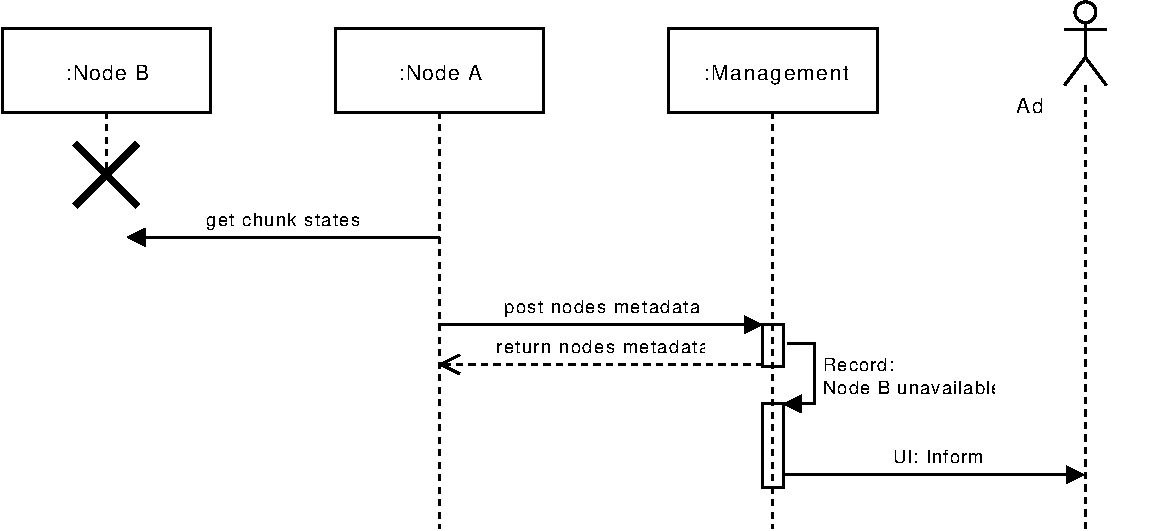
\includegraphics[width=\linewidth]{resources/node_leaving_unplanned.pdf}
    \caption{Node Leaving Unplanned Sequence Diagram}
    \label{fig:node-leave-unplanned}
\end{figure}

This scenario is described as it is implemented in the study project. It might be subject to further evaluation in the future.

\begin{enumerate}
    \item If a node is not responding (which means, no other node nor the management can reach it), the management records the unavailability and informs the administrator.
    %Replikationsmechanismus; management knows, that on reason of intervall the node is away
\end{enumerate}

\begin{itemize}
    \item If the node returns, then the node carries on.
    \item If the administrator marks the node as \emph{left}, which will be propagated to all nodes via the \emph{node fetch all nodes metadata} message.
        \begin{itemize}
            \item Data, which was not previously replicated from the node are lost.
        \end{itemize}
\end{itemize}

\subsubsection{Data Replication}\label{sec:scenario-data-replication}
The network distributes backup data.

\begin{figure}[h]
    \centering
    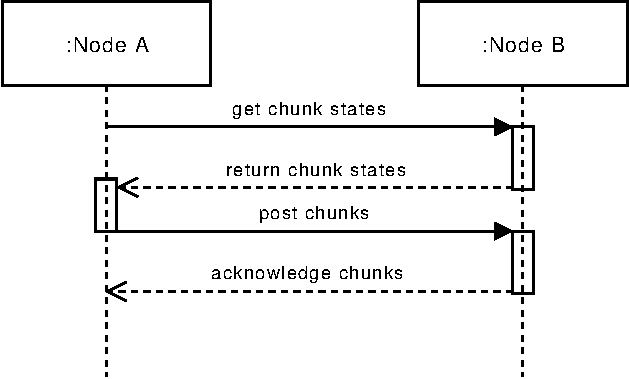
\includegraphics[width=0.6\linewidth]{resources/data_replication.pdf}
    \caption{Data Replication Sequence Diagram}
    \label{fig:data-replication}
\end{figure}

This scenario is described as it is implemented in the study project. It might be subject to further evaluation in the future.

\begin{enumerate}
    \item The sending node picks $n$ random entries from its \emph{node chunk table}. In the future, the chunks might be selected based on heuristics.
    \item The sending node picks one random designated node from its \emph{node metadata table}. In the future, the nodes might be selected based on heuristics. %TODO: naming of node metadata table could be better ;)
    \item The sending node sends the chosen \emph{chunk identifier}s to the designated node with a \emph{client sends chunk list} %TODO: Rename. Can be the samme message as for the client?
    \item The designated node checks, if all chunks received from the sending node are present in its \emph{node chunk table}
        \begin{itemize}
            \item If a chunk is already present, update its expiration date if it is further in the future.
            \item If a chunk is not present, request it from the \emph{sending node} (see message response \emph{client sends chunk list} for further details).
        \end{itemize}
    \item The sending node sends the \emph{requested chunks} to the \emph{designated node} with a \emph{client sends chunk} message. %TODO: Rename. the. message.
        \begin{itemize}
            \item The \emph{designated node} verifies and persists the chunk into its \emph{storage}. Afterwards, it acknowledges receipt to the \emph{sending node} (see \emph{client sends chunks} message).
        \end{itemize}
\end{enumerate}

\subsubsection{Data has Expired Lifetime}\label{sec:scenario-data-expiration}
A node wants to delete data associated with an expired backup/snapshot.

This scenario is described as it is implemented in the study project. It might be subject to further evaluation in the future.

\begin{itemize}
    \item The \emph{management} monitors the nodes physical timestamp and records any deviation from the management time larger than 1h.
    \item Therefore, a first prototype, the system may just delete chunks after the specified keep date without further checks.
        \begin{itemize}
            \item We build on the assumption, that the nodes have different upstream timeservers, so that a general time shift is unlikely.
            \item In case a single node's time is in the past, and runs out of storage, it might lead to a degraded system (redundancy loss).
            \item If a single nodes time is in the future, the redundancy is reduced by one.
        \end{itemize}
\end{itemize}

In the future, it is advisable to implement a consent protocol to reduce the likelihood of data loss.

\subsubsection{Data Storage has Errors}\label{sec:scenario-storage-errors}
The storage layer notifies the node that some of the data stored on it is corrupt.

This scenario is described as it is implemented in the study project. It might be subject to further evaluation in the future.

\begin{enumerate}
    \item The storage informs the node of a corrupt data set
    \item The node removes the \emph{chunk identifier} from the \emph{node chunk table}.
        \begin{itemize}
            \item The chunk will be replicated eventually.
        \end{itemize}
    \item On the next \emph{node fetch all nodes metadata} request to the management.
\end{enumerate}

\subsubsection{Management Problems}\label{sec:scenario-management-problems}
\begin{itemize}
    \item The case, that the management has outdated metadata out of a data loss, will be ignored during this study project. A mechanism solving this problem, would probably be subject to significant changes in further system development e.g.\ when implementing limited redundancy levels. %TODO: Counter in config in the future
\end{itemize}

\subsubsection{Network Availability Problems}\label{sec:scenario-network-errors}
\paragraph{Behaviour in case a node can reach only some nodes directly}
The still available nodes should try to satisfy redundancy needs as good as possible.
If a node cannot reach other nodes, it notifies the management with the next \emph{node fetch all nodes metadata}

\paragraph{Behaviour in case the network gets partitioned}
(, and the nodes in each partition can only reach each other and not the other ones.)

See first case in scenario~\ref{sec:scenario-network-errors}

\paragraph{Behaviour in case nodes have different states of management information}
The redundancy is temporary reduced to the nodes, which the group of old nodes know, but will eventually be resolved as nodes fetch \emph{metadata}. %TODO: rename metadata